\documentclass[12pt]{article}

\usepackage{tgtermes} 
\usepackage{verbatim}
\usepackage{graphicx, float}
\usepackage{enumerate}
\usepackage{amsmath}
\usepackage[margin=1in]{geometry}
\usepackage{hyperref}

\author{Astrid Augusta Yu}
\title{EE 143-08 Lab \#3}

\begin{document}
\begin{titlepage}
    \centering
    {
    \large
    Instructor: Aiku Shintani 
    \vspace{.25cm}
    
    EE 143 Section 08 \par \vspace{.2cm}\par
    T 6:10-9PM    
    }
    
    \vfill
    
    { \Huge Experiment 3 \par }
    { \Large
    R, V \& I Measurement \par Ohm's Law, KCL and KVL \par Accuracy and Precision \par Reverse Engineer a PCB \par
    }
    
    \vfill
    
    \includegraphics[width=0.78\textwidth]{revsch.png}\par\vspace{1cm}  
    \vfill
    
    {\large 
    Written by Astrid Yu\par
    \today}
\end{titlepage}

\section*{Introduction}

The purpose of this experiment is to learn how to read resistors and use a multimeter.
An additional purpose is to learn about accuracy an resolution, to verify electrical laws
(such as Ohm's Law, KCL, and KVL), and to understand open circuits and shorts, as well as 
to understand what a node is and to draw a schematic from a PCB.

\section*{Analysis}

\subsection*{1. Accuracy and Precision}

\begin{figure}[H]
    \centering
    \includegraphics[width=0.3\linewidth]{multimeter.jpg}
    \caption{A Neoteck NT8233D Pro.}
    \label{fig:multimeter}
\end{figure}
\begin{enumerate}[a)]
    \item The multimeter used is a Neoteck NT8233D Pro, pictured in Figure \ref{fig:multimeter}. 
        According to the manufacturer's website, the multimeter has the following precision steps: 
        \begin{table}[H]
            \label{tbl:mmsteps}
            \centering
            \caption{Neoteck NT8233D Pro precision steps. (Source: \url{http://www.neoteck.cn/index.php/2017/03/16/ntk017/})}
            \begin{tabular}{c c}
                \hline
                Measurement Type & Steps \\
                \hline
                Voltage & $200mV, 2V, 20V, 200V$ \\ 
                Current & $200\mu A, 2000\mu A, 20mA, 200mA, 10A$ \\
                Resistance & $200\Omega,2k\Omega,20k\Omega,200K\Omega$ \\
                \hline 
            \end{tabular}
            
        \end{table}
        It has an auto-ranging feature, which is its only mode 
        of ranging (no manual ranging). 
    
    \item This step was skipped because the multimeter only has auto-ranging.
    \item A $470\Omega$ resistor was measured, with results in the table below.
        \begin{table}[ht]
            \label{tbl:470res}
            \caption{Measurement of a $470\Omega\pm 5\%$ resistor}
            \centering
            \begin{tabular}{| c | c |}
                \hline
                Best Precision Range & Auto Range Readout ($\Omega$) \\
                \hline
                $2k\Omega$ & $0.459 k\Omega$  \\
                \hline
            \end{tabular} 
        \end{table}
    
    \item The resistance of the leads was measured to be $0.0\Omega$ on the $200\Omega$ range (the smallest).
\end{enumerate}
    
\subsection*{2. Body Resistance Measurement}
\begin{enumerate}[a)]
    \item Probes were held between the thumb and forefinger of each hand, and the 
        resistance of Astrid's body was measured.
    \item This was repeated again after moistening the thumb and forefinger.
\end{enumerate}
\begin{table}[ht]
    \caption{Measurement of body resistance}
    \label{tbl:bodyres}
    \centering
    \begin{tabular}{| c | c | c |}
        \hline
        Name & Body Resistance, Dry Fingers & Body Resistance, Moist Fingers \\
        \hline
        Astrid & $0.805 M\Omega$ & $0.317 M\Omega$ \\
        \hline
    \end{tabular} 
\end{table}

\subsection*{3. Reverse Engineering a PCB Layout}

\begin{figure}[H]
    \centering
        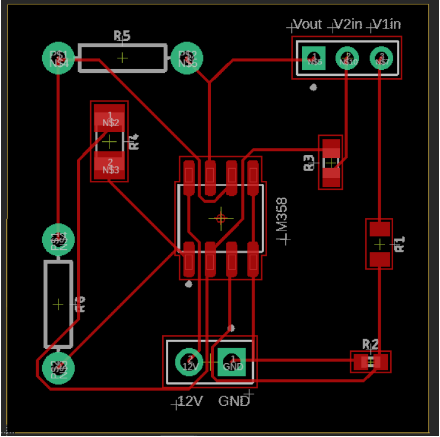
\includegraphics[width=0.5\linewidth]{pcb.png}
    \caption{The PCB that was reverse engineered.}
    \label{fig:revengpcb}
\end{figure} 

The PCB layout in Figure \ref{fig:revengpcb} was analyzed and reverse-engineered. The 
in Figure \ref{fig:revsch} was produced in EAGLE 

\begin{figure}[H]
    \centering
    
    \includegraphics[width=0.7\linewidth]{revsch.png}
    
    \caption{Reverse-engineered schematic made in EAGLE. The LM358 symbol only had 
    one pair of VCC and GND, which is why they only exist on one op-amp.}
    \label{fig:revsch}
\end{figure}

\subsection*{4. Verification of Kirchhoff's Circuit Laws}

\begin{figure}[H]
    \centering
    \includegraphics[width=0.4\linewidth]{ctestsch.png}
    \caption{The continuity tester schematic.}
    \label{fig:ctestsch}
\end{figure}

\begin{enumerate}[a)]
    \item The circuit pictured in Figure \ref{fig:ctestsch} was reproduced on a breadboard,
        as seen in Figure \ref{fig:sec4setup}. An Arduino was used as the power supply, and 
        the basic functionality of the continuity tester (LED lighting up when connected, and 
        shutting off when disconnected) was verified.

    \item Next, X and Y were shorted together.
    \item A voltmeter was used to verify KVL along Loop 1 and Loop 2. The voltage drops are listed
        in Tables \ref{tbl:loop1} and \ref{eqn:loop2} respectively, and the mathematical verification 
        of KVL is in equations \ref{eqn:loop1} and \ref{eqn:loop2} respectively.

        \begin{figure}[H]
            \centering
            \includegraphics[width=0.4\linewidth]{setup.jpg}
            \caption{The experimental setup used to test the continuity tester.}
            \label{fig:sec4setup}
        \end{figure}

        \begin{table}[ht]
            \caption{Voltage drops along Loop 1 when X and Y are shorted}
            \label{tbl:loop1}
            \centering
            \begin{tabular}{| c | c | c | c | c |}
                \hline
                V($5V$ source) & V(diode) & V(R2 = $10k\Omega$) & V(R3 = $100\Omega$) & V(R5 = $100\Omega$) \\
                \hline
                $4.99V$ & $0.723V$ & $3.84V$ & $193.5mV$ & $0.234V$ \\
                \hline 
            \end{tabular}
        \end{table}

        Equation \ref{eqn:loop1} demonstrates that KVL holds true for Loop 1.

        \begin{equation}
            \label{eqn:loop1}
            \begin{split}
                & V(5V \textnormal{source}) - V(\textnormal{diode}) - V(R2 = 10k\Omega) - V(R3 = 100\Omega) \\ & - V(R5 = 100\Omega)  \\
                = & 4.99V - 0.723V - 3.84V - 193.5mV - 0.234mV \\
                = & 233.266mV \\
                \approx & \textbf{0V}
            \end{split}
        \end{equation}

        \begin{table}[ht]
            \caption{Voltage drops along Loop 2 when X and Y are shorted}
            \label{tbl:loop2}
            \centering
            \begin{tabular}{| c | c | c | c | c |}
                \hline
                V($5V$ source) & V(diode) & V(R4 = $470\Omega$) & V(LED) & V(Pin 7) \\
                \hline
                $4.99V$ & $0.723V$ & $2.19V$ & $1.918V$ & $155.1mV$ \\
                \hline 
            \end{tabular}
        \end{table}

        Equation \ref{eqn:loop2} demonstrates that KVL holds true for Loop 2.

        \begin{equation}
            \label{eqn:loop2}
            \begin{split}
            & V(5V source) - V(diode) - V(R4 = 470\Omega) - V(LED) - V(Pin 7) \\
            = & 4.99V - 0.723V - 2.19V - 1.918V - 155.1mV \\
            = & 3.9mV \\
            \approx & \textbf{0V}
            \end{split}
        \end{equation}
    \item An ammeter was used to verify KCL at node A for when there is both an open and 
        a short between X and Y. The currents entering and leaving are listed in Table 
        \ref{tbl:nodea}.
        \begin{table}[ht]
            \centering
            \caption{Current entering and exiting Node A}
            \label{tbl:nodea}
            \begin{tabular}{| c | c | c | c | c | c |}
                \hline
                X and Y & I(diode) & I(R1 = $2k\Omega$) & I(R2 = $10k\Omega$) & I(R4 = $470\Omega$) & I(Pin 8) \\
                \hline
                Disconnected & 3.12mA & 0.0$\mu A$ & 1922 $\mu A$ & 0.0$\mu A$ & 1112 $\mu A$ \\
                \hline
                Connected & 9.49mA & 403 $\mu A$ & 1873 $\mu A$ & 4.74mA & 2.40mA \\
                \hline  
            \end{tabular}
        \end{table}

        Equation \ref{eqn:node1} demonstrates that KCL holds true for Node A when X and Y are disconnected.

        \begin{equation}
            \label{eqn:node1}
            \begin{split}
                & I(diode) - I(R1 = 2k\Omega) - I(R2 = 10k\Omega) - I(R4 = 470\Omega) - I(Pin 8) \\
                = & 3.12mA - 0.0\mu A - 1922 \mu A - 0.0\mu A - 1112 \mu A \\
                = & 86\mu A \\
                \approx & \textbf{0A}
            \end{split}
        \end{equation}

        Equation \ref{eqn:node2} demonstrates that KCL holds true for Node A when X and Y are connected.

        \begin{equation} 
            \label{eqn:node2}
            \begin{split}
                & I(diode) - I(R1 = 2k\Omega) - I(R2 = 10k\Omega) - I(R4 = 470\Omega) - I(Pin 8) \\
                = & 9.49mA - 403 \mu A - 1873 \mu A - 4.74mA - 2.40mA \\
                = & 74\mu A \\
                \approx & \textbf{0A}
            \end{split}
        \end{equation} 
\end{enumerate}


\section*{Discussion}

\subsection*{Section 1}

\begin{enumerate}
    \item {
        \textit{Generally, which multi-meter range yields the best precision?}
        
        The range with the smallest limits yields the best precision.
    } 
\end{enumerate}

\subsection*{Section 2}

\begin{enumerate}
    \setcounter{enumi}{1}
    \item {
        \textit{Contrast your body resistance with dry fingertips compared to your body resistance
        with damp fingertips. For a given amount of voltage, when are you more susceptible to serious
        injury due to electricity? Use Ohm's Law to support your answer. ($6mA$ causes painful shock 
        and $50mA$ is fatal.)}

        By Ohm's Law, $I = \frac{V}{R}$, to maximize $I$ and cause injury for a constant $V$, $R$ 
        must be decreased. According to Table \ref{tbl:bodyres}, Astrid is a better conductor 
        when her fingers are moist, so she is more susceptible to injury when wet than dry.
    }
\end{enumerate}

\subsection*{Section 3}

\begin{enumerate}
    \setcounter{enumi}{2}
    \item {
        \textit{Draw a box/rectangle around each of the nodes on your schematic. Insert a picture of
        schematic here.}
       
        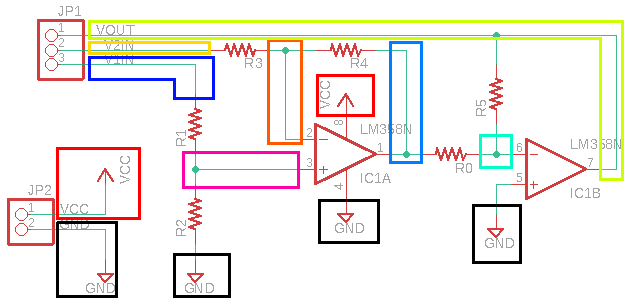
\includegraphics[width=.8\linewidth]{revsch-nodes.png}
        
        Each color is its own node. The 12V and GND ports are all connected together and thus each count as a 
        single node.
    }  
    \item {
        \textit{How many nodes are there in the schematic?}

        There are 9 nodes in the schematic.  
    }
\end{enumerate}

\subsection*{Section 4}

\begin{enumerate}
    \setcounter{enumi}{4}
    \item {
        \textit{Explain the difference in diode current when there's an open in the continuity-tester leads 
        and when there's a short between the leads.}
        
        The LED is not being powered, so there is less voltage being supplied to the circuit through the diode.
    }   
    \item{
        \textit{Write the KVL equation for the loop containing the $5V$ source, diode, and $2k\Omega$ 
        resistor when there is an open between the continuity leads. What is the voltage across the open?}
    
        The op-amp is in an open-loop amplifier configuration, so the voltage difference between the positive and 
        negative leads \textit{is not} negligible.

        Let $\Delta V = $ the voltage across the open between X and Y. The KVL equation is the following:
        \begin{equation}
            \label{eqn:sec4kvl}
            V(5V source) - V(diode) - V(R1) - \Delta V - V(R5) = 0  \\
        \end{equation}

        The following values are known:
        \begin{equation}
            \begin{aligned}
                V(5V source) &= 5V && \text{By definition} \\
                V(diode) &= 0.7V && \text{Assumed} \\
                V(R1) &= 0V && \text{Only attached on 1 end} \\
                V(R5) &= 5V \frac{100\Omega}{10k\Omega + 100\Omega + 100\Omega}  && \text{Voltage divider} \\
                &\approx 9.80mV
            \end{aligned}
        \end{equation}

        Substituting these values into equation \ref{eqn:sec4kvl} and rearranging:
        \begin{equation}
            \begin{aligned}
                5V - 0.7V - 0V - \Delta V - 9.80mV &= 0 \\
                \Delta V &= \textbf{4.29V} 
            \end{aligned}
        \end{equation}
    }
    \item {
        \textit{Using the data from procedure steps c and d, how much power is expended by the LED when lit?}
     
        The LED and R4 are connected in series. Therefore, $I(R4) = I(LED)$.
        \begin{equation}
            \begin{aligned}
                I(LED) &= I(R4) = 4.74mA && \textnormal{(see table \ref{tbl:nodea})} \\
                V(LED) &= 1.918V && \textnormal{(see table \ref{tbl:loop2})} \\
                P(LED) &= I(LED) \times V(LED) \\ 
                &= (4.74mA)(1.918V) \\ 
                &= \textbf{9.09mW}
            \end{aligned}
        \end{equation}

    }
    \item {
        \textit{In step (e), did the LED glow brighter or dimmer after the $470\Omega$ resistor was replaced 
        with a $20k\Omega$ resistor? Explain with your knowledge of Ohm's Law.}
        
        The LED was dimmer after the resistor was replaced with a stronger one. By Ohm's Law, resistance is inversely proportional
        to current for constant voltage. With more resistance, there is less current flowing, which results in 
        less power delivered to the LED.
    }
\end{enumerate}

\section*{Conclusion}

This experiment was successful. The error of a resistor and a multimeter was observed, human body resistance 
was quantified, a PCB was reverse-engineered and analyzed, and Kirchhoff's current and voltage laws were verified 
multiple times.

The measured voltage drops and current flows were underestimates, as shown by equations \ref{eqn:loop1}, 
\ref{eqn:loop2}, \ref{eqn:node1}, and \ref{eqn:node2} all having positive residuals before being rounded down 
to zero. In the case of equations \ref{eqn:loop1} and \ref{eqn:loop2}, the KVL equations, this is because there is 
lead resistance creating a voltage divider and reducing the observed voltage. In the case of equations \ref{eqn:node1}
and \ref{eqn:node2}, the KCL equations, even though the multimeter's resistance is small, it is still
somewhat present, reducing the amount of current flowing through the individual branches. 

\end{document}
